%======================================================================
\chapter{Introduction}
%======================================================================

Risk management is a key component of modern financial systems.
Successful risk management practice can enhance financial stability and resilience for individual companies and for the financial system as well.
\gls{va} contracts are a popular type of complex insurance product that is linked to the performance of underlying assets.
They provide a guaranteed minimum income benefit to the policyholder regardless of the performance of the underlying assets.
Advanced Monte Carlo simulation techniques, particularly nested simulation procedures, become indispensable for risk assessment of such products.
In contrast to finite-difference methods, a Monte Carlo simulation scheme is more flexible and can be easily adapted to model tail risk with a rule-based design.
~\cite{glasserman2004monte} provide a comprehensive overview of Monte Carlo simulation methods in financial engineering and risk management applications.
In this thesis, we focus on building and analyzing nested simulation procedures for risk management applications of financial derivatives and insurance products.
Nested simulation, also known as nested stochastic modeling and stochastic-on-stochastic modeling, becomes a necessary tool when stochastic simulation of a parameter of interest is contingent on another quantity to be determined stochastically.
In the context of financial engineering, nested simulation is used to model the tail risk of a contract whose payoff depends on a set of underlying risk factors.
For example, estimating the value of an exotic option over a risk horizon requires simulation given a realization of the underlying assets over that horizon.
A standard nested simulation procedure consists of two levels of simulation: the outer-level simulation generates the underlying risk factors, while the inner-level simulation estimates the value of interest with the inner sample mean from another level of Monte Carlo simulation.
This nested structure allows for accurate estimation given sufficient computational resources, but it also introduces additional complexity in the simulation design and implementation.
Furthermore, in real-world applications, the computational burden of a nested simulation can be prohibitive.
The number of inner simulations required to achieve a desired level of accuracy for each outer scenario can be large.
Metamodeling techniques can reduce the computational burden of nested simulations by approximating the inner simulation model.
Metamodels are statistical models that approximate the output of a complex simulation model as a function of its input parameters.
In this thesis, we focus on metamodels of the inner simulation models in nested simulation procedures for risk management applications of financial derivatives and \gls{va} contracts.
This thesis addresses two key problems that necessitate nested simulation:
\begin{itemize}
    \item estimating the risk of a portfolio of financial options and 
    \item dynamic hedging of \gls{va} contracts with a delta hedging strategy.
\end{itemize}
Risk management of VAs is a challenging problem due to the complex interactions between the policyholder's behavior and the financial market dynamics.
We focus mainly on the estimation of tail risk measures of \gls{va} contract losses using metamodel-based nested simulation procedures.
This thesis consists of four chapters.
Chapter \ref{chap:project1} summarizes theoretical convergence results of several state-of-the-art single-period nested simulation procedures under the same analytical framework.
Numerical experiments are conducted to test their empirical convergence behavior under finite budget sizes.
Chapter~\ref{chap:project2} proposes the use of neural network models as metamodels for a two-stage multi-period nested simulation procedure on \gls{va} contracts.
In our numerical experiment, the best neural network metamodel surpasses the state-of-the-art metamodels in tail identification, and it leads to substantial computational savings.
Chapter~\ref{chap:project2} also includes sensitivity testing of the neural network metamodel.
We argue that for estimating tail risk measures of \gls{va} contract losses, the inner simulation can be replaced entirely by a suitable metamodel.
Eliminating the inner simulation can lead to more substantial computational savings without affecting estimation quality.
When extensive inner simulations are required for regulatory purposes, effective budget allocation can improve estimator accuracy without increasing the computational budget.
In practice, underlying assumptions of the simulation model are subject to change, and new \gls{va} contracts are issued with different contract specifications.
Simulation budgets are often scarce for new conditions.
Chapter~\ref{chap:project3} uses transfer learning techniques for a quick adaptation of the neural network metamodel to new market conditions and new \gls{va} contracts.
Our numerical experiments show that a judicious use of transfer learning can lead to substantially better metamodels than those trained from scratch.
Chapter~\ref{chap:conclusion} concludes this thesis and discusses potential future research directions.
Chapter~\ref{chap:futureWork} explores future applications of deep reinforcement learning in the dynamic hedging of \gls{va} contracts.

\section{Risk Management of Variable Annuities with Nested Simulation}

\gls{va} contracts are index-linked insurance products that offer policyholders the upside potential of equity markets while providing guarantees against downside risk.
These products have gained a substantial amount of interest as they address the needs of individuals seeking both wealth accumulation and financial security, especially in the context of retirement planning.
The key feature of VAs is their embedded guarantees, which ensure a specified minimum benefit regardless of market performance.
Two \gls{va} contracts that are most relevant to this thesis are \gls{gmmb} and \gls{gmwb}.
The \gls{gmmb} guarantees that at the maturity of the contract, the policyholder will receive no less than the initial investment or a predetermined minimum amount.
The \gls{gmwb} allows policyholders to withdraw a specified percentage of their benefit base each period during the contract horizon~\citep{hardy2003investment}.
While these guarantees make VAs more attractive to consumers by offering protection against market downturns and ensuring income stability, they also introduce significant financial risks for insurers.
The embedded options within \gls{gmmb} and \gls{gmwb} expose insurers to market risk, longevity risk, and policyholder behavior risk.
Therefore, an effective management of these risks is crucial for insurers to maintain solvency and meet regulatory capital requirements.

One of the primary risk management strategies employed by insurers to mitigate the financial risks associated with VAs is dynamic hedging.
Dynamic hedging involves frequent adjustments to a portfolio of financial instruments to offset changes in guarantee values due to market movements~\citep{hull2016options}.
This strategy aims to neutralize the insurer's liability sensitivity to market fluctuations by constructing a hedging portfolio that replicates the guarantees' cash flows.
However, dynamic hedging introduces complexity in estimating the insurer's overall risk exposure.
One such example is the estimation of tail risk measures of a \gls{va} contract.
It requires a stochastic modeling of the financial market and an accurate loss estimation of the hedging portfolio under different market scenarios.
Nested simulation is a robust method for estimating risk measures in complex settings~\citep{gordy2010nested}.
In nested simulation, an outer simulation generates a set of market scenarios over the contract horizon, while an inner simulation estimates the contract loss in each scenario.
By combining the results of the inner simulations across the outer scenarios, nested simulation provides an accurate estimate of the tail risk of the \gls{va} contract.

Despite its robustness, nested simulation is computationally intensive, often demanding significant computational resources and time.
Each outer simulation scenario requires numerous inner simulations to accurately estimate contract loss.
This computational burden poses practical limitations, especially when a high degree of precision in tail risk estimation is required.
To address this challenge, metamodeling techniques can be employed to approximate the inner simulation model and reduce the computational cost of nested simulation.

\section{Metamodeling for Monte Carlo Simulation}

Metamodeling, or surrogate modeling, approximates complex simulation models with simpler, computationally efficient models.
In Monte Carlo simulations, metamodels reduce computational costs by approximating simulation outputs based on input variables~\citep{kleijnen2018design}.
This section introduces metamodeling for a Monte Carlo simulation, elaborates on its methodologies, and highlights its importance in practical applications.

Monte Carlo simulations are widely used for modeling and analyzing complex systems that are probabilistic in nature.
These simulations often require a substantial amount of computational resources, especially when a high degree of accuracy or a high number of iterations is necessary~\citep{glasserman2004monte}.
Metamodeling addresses this challenge by constructing an approximate model (known as a metamodel) that emulates the behavior of the original simulation model with much less computational effort.
The metamodel serves as a predictive model that maps input variables to output responses.
Learning from a set of simulation runs, the metamodel can generalize and predict outputs for new inputs without running the full simulation.
Metamodeling is especially useful for computationally expensive simulation models.
Replacing the simulation model with a metamodel significantly reduces computational costs.
This allows for faster convergence of simulation-based estimators.

The process of metamodeling generally involves the following steps:

\begin{enumerate} 
    \item \textbf{Design of Experiments}: Select input combinations to run the original simulation and collect data.
    \item \textbf{Building the Metamodel}: Use the collected data to train a metamodel that approximates the simulation model.
    \item \textbf{Validation}: Assess the metamodel's accuracy and generalization capability.
    \item \textbf{Application}: Use the metamodel to predict simulation outputs for new input combinations.
\end{enumerate}

The development of advanced machine learning models and deep learning techniques has enhanced metamodeling approaches for Monte Carlo simulations, especially in high-dimensional and complex problem settings.
Examples of machine learning applications include~\cite{jin2020deep},~\cite{tang2020deep}, and~\cite{rosen2012metamodeling}.
These methods offer powerful tools for capturing intricate patterns and nonlinear relationships that traditional metamodeling techniques might struggle to model effectively.
In the following sections, we discuss machine learning algorithms in the context of metamodeling for Monte Carlo simulations and their applications in risk management.

\section{Machine Learning for Risk Management Applications}

Machine learning (ML) algorithms are essential tools for identifying complex patterns and relationships in data.
In particular, they are well-suited for handling non-linearities and large-scale data structures, which are challenging for traditional statistical methods.
In the context of risk management, ML algorithms have been widely used for predicting financial time series, estimating risk measures, and optimizing trading strategies.
ML algorithms can be broadly categorized into supervised learning, unsupervised learning, and reinforcement learning.
This section focuses on three widely used supervised learning models and two reinforcement learning algorithms that are most relevant to risk management applications.

\subsection{Supervised Learning Models}

Supervised learning is a fundamental approach in machine learning where the algorithm learns a mapping from inputs to outputs based on example input-output pairs~\cite{galton1886regression}.
In this paradigm, a model is trained on a labeled dataset, which means that each training example is associated with an output label or value.
The goal of a supervised learning paradigm is to learn a general rule that maps inputs (also known as features) to outputs (also known as targets), enabling the model to make accurate predictions on new, unseen data.
Supervised learning is usually applied in two domains:
\begin{itemize} 
    \item \textbf{Classification}: The output variable is categorical, and the task is to assign inputs to one of several predefined categories to produce a qualitative prediction.
    Common uses in finance and actuarial applications are fraud detection and credit scoring.
    \item \textbf{Regression}: The output variable is continuous, and the task is to predict a real-valued number and produce a quantitative prediction.
    Examples in actuarial applications include predicting claim amounts, reserve estimates, asset pricing, and estimating tail risk measures of loss distributions.
\end{itemize}

This thesis focuses on regression models for risk management applications, where the goal is to predict a continuous target variable based on one or more input features.
Given a dataset of $n$ observations $\{(x_1, y_1), (x_2, y_2), \ldots, (x_n, y_n)\}$, where $x_i \in \mathbb{R}^d$ is the $d$-dimensional input feature vector, and $y_i \in \mathbb{R}$ is the target variable, a supervised learning algorithm aims at learning a function $f(x;\theta): \mathbb{R}^d \mapsto \mathbb{R}$ that to predict $y$ from $x$ using parameters $\theta$.

Linear regression, kernel regression, and neural networks all fall under the supervised learning category and are widely used in risk management applications.
Despite the differences in their functional forms, all supervised learning models can be evaluated on a similar set of metrics.
The learning process, called training, minimizes a loss function $l(f(x; \theta),y)$ over the training data, which quantifies the difference between predicted and actual labels.
A common loss function for regression problems is a quadratic loss function in the form of a \gls{mse}:

\begin{equation} \label{eq:mse}
    \text{MSE} = \frac{1}{n} \sum_{i=1}^{n} (f(x_i;\theta) - y_i)^2.
\end{equation}

In most risk management applications, a critical task of users of supervised learning models is to design a suitable loss function that aligns with the objectives of the problem.
Another important consideration is the choice of a suitable supervised learning algorithm.
The choice may vary based on a trade-off among the complexity of the relationship, the interpretability of the model, and the computational resources available.
In the following sections, we discuss four widely used supervised learning techniques in risk management applications: parametric regression, kernel regression, and two neural network architectures.

\subsection{Parametric Regression Models}

Regression models are the most common supervised learning algorithms used in risk management applications.
A regression model predicts a continuous target variable based on one or more input features.
A multiple linear regression is a simple and interpretable model that attempts to predict a target variable as a linear combination of input features.
It assumes a linear relationship between the target output and one or more input features.
This method has been thoroughly explored in statistical literature.
\citet{bishop2006pattern} provide an extensive treatment of regression techniques in the broader context of machine learning.
It is known as a parametric regression because it assumes a specific functional form for the input-output relationship with a finite set of parameters~\citep{seber2012linear}.
A general form of a parametric regression model is given by:
\begin{equation} \label{eq:regression}
    f(x; \theta) = \beta_0 + \sum_{j=1}^{p} \beta_j \phi_j(x),
\end{equation}
where $p$ is a number of features, $\beta_0, \beta_1, \ldots, \beta_p$ are trainable regression coefficients, and $\phi_j(x)$ are basis functions that transform the input $x$ to allow for non-linear modeling.
Basis functions can be any functions of $x$ that are chosen to capture the underlying structure of the data.
Common choices include polynomial basis functions: $\phi_j(x) = x^j$ and Laguerre basis functions: $\phi_j(x) = e^{-x/2} L_j(x)$, where $L_j(x)$ are the Laguerre polynomials that are solutions to the Laguerre differential equation~\citep{szeg1939orthogonal}.
The training of parametric regression refers to the process of estimating the regression coefficients $\beta_0, \beta_1, \ldots, \beta_p$ that minimize the loss function.
For a \gls{mse} loss metric, the optimal regression coefficients can be obtained by solving the normal equations.
Parametric regression is powerful for modeling linear relationships when basis functions are known from expert knowledge or feature engineering~\citep{hastie2009elements}.
These techniques utilize predefined functional forms to model the relationship between a set of independent variables and a dependent variable.
However, when data exhibits complex, non-linear relationships, linear models fall short.
While these methods are straightforward and interpretable, they impose strong assumptions about the underlying data structure.
Often, expert knowledge is required to select the appropriate basis functions, which can limit the flexibility of the model.
Extensions like polynomial regression and \gls{glm} have been introduced to capture non-linearity in the data.
Nevertheless, these models can still be limited in capturing highly complex patterns of the data.

\subsection{Non-Parametric Regression Models}
To overcome some of the previously mentioned limitations of parametric regression methods, non-parametric methods such as kernel regression~\citep{hastie2009elements} are often employed.
Kernel regression estimates the relationship by averaging the values of the target variable over a local neighborhood of the input $x$.
The kernel regression with the Nadaraya-Watson estimator is given by:
\begin{equation}
    f(x; \theta) = \frac{\sum_{i=1}^{n} K\left(\frac{x-x_i}{h}\right) y_i}{\sum_{i=1}^{n} K\left(\frac{x-x_i}{h}\right)},
\end{equation}
where $K(\cdot)$ is a kernel function, which assigns weights to the data points based on their distance to the input $x$, and $h$ is a bandwidth parameter that controls the smoothness of the estimated function.
The objective of this approach is to estimate a feature-label relationship directly from the data without imposing a specific functional form of the regression function.
However, they come with several drawbacks that limit their effectiveness, especially in high-dimensional settings or for large datasets.
One of the most important drawbacks of non-parametric regression methods is the curse of dimensionality~\cite{bellman1966dynamic}.
As the number of features increases, the volume of the input space grows exponentially.
Data points become sparse and the model may overfit to noise in the data.
In addition, the computational cost associated with non-parametric methods often grows rapidly with the number of dimensions.
Cross-validation and distance calculations are computationally expensive for non-parametric regression.
These drawbacks render non-parametric regression impractical for high-dimensional, large-scale datasets.

\subsection{Feedforward Neural Networks}

The progression from traditional parametric and non-parametric regression methods to neural network architectures has been driven by the need to model increasingly complex and high-dimensional data.
Neural networks are powerful tools that overcome many limitations of traditional regression methods.
They can learn complex, non-linear relationships in data without the need for explicit feature engineering.
The most basic form of a neural network is the \gls{fnn}, which consists of an input layer, one or more hidden layers, and an output layer~\citep{goodfellow2016}.

\begin{figure}[ht!]
    \centering
    \begin{subfigure}{0.45\textwidth}
        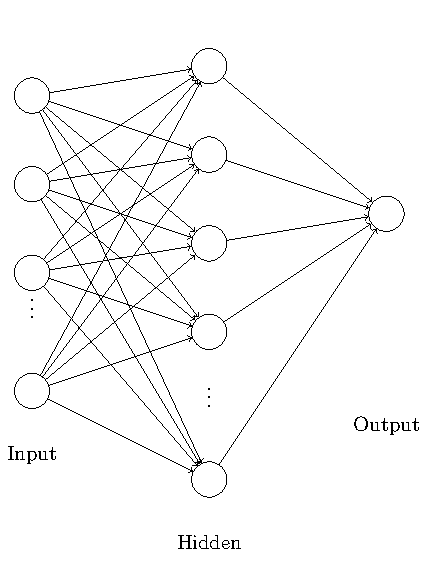
\includegraphics[width=\textwidth]{./project3/tikz/fnn.pdf}
        \caption{\gls{fnn}}
        \label{subfig:fnn}
    \end{subfigure}
    \hspace{1cm}
    \begin{subfigure}{0.45\textwidth}
        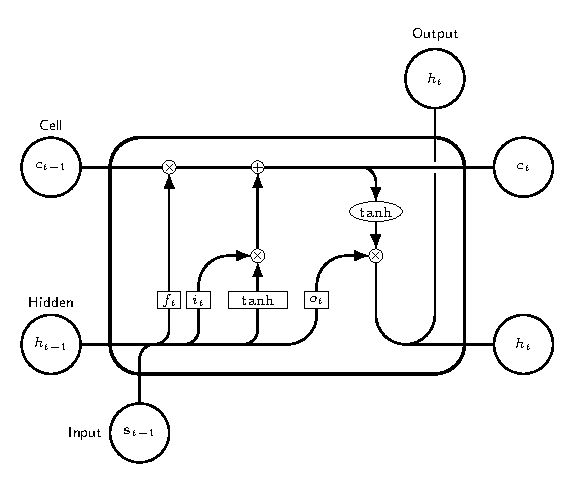
\includegraphics[width=\textwidth]{./project3/tikz/lstm.pdf}
        \caption{\gls{lstm}}
        \label{subfig:lstm}
    \end{subfigure}
    \caption{Neural Network Architectures}
    \label{fig:nn}
\end{figure}

Figure~\ref{subfig:fnn} shows a \gls{fnn} architecture with one hidden layer.
The input layer receives the input features, which are then passed through the hidden layer(s) to the output layer.
Each layer consists of multiple neurons, which apply a non-linear activation function to the weighted sum of the inputs.

\begin{equation}
    f(x; \theta) = f^{(k)}(f^{(k-1)} \cdots (f^{(2)}(f^{(1)}(x;\theta^{(1)});\theta^{(2)} )\cdots ;\theta^{(k-1)});\theta^{(k)}),
\end{equation}
where $\theta = (\theta^{(1)}, \theta^{(2)}, \ldots, \theta^{(k)})$ are trainable parameters of the neural network, $f^{(i)}$ is an $i$-th layer of the neural network, $x$ is an input feature vector, $f^{(1)}(x;\theta^{(1)}) = x$, $f^{(k)}$ is an output layer, $k$ is a number of layers, and $f^{(i)}$ is an output of the $i$-th layer.
To transition from layer $i-1$ to layer $i$,
\begin{equation} \label{eq:neural}
    f^{(i)}(z;\theta^{(i)}) = a^{(i)}(\beta_0^{(i)} + \sum_{j=1}^{p_i} \beta_j^{(i)} z),
\end{equation}
where $a^{(i)}$ are nonlinear activation functions, $\theta^{(i)} = (\beta_0^{(i)}, \dots, \beta_p^{(i)})$ are trainable parameters of the $i$-th layer, and $p_i$ is a number of neurons in the previous layer.
Equation~\eqref{eq:neural} represents a single neuron in a neural network, which applies a linear transformation to the input followed by a non-linear activation function.
The linear transformation is similar to the linear regression model in Equation~\eqref{eq:regression}, but the non-linear activation function allows the neural network to model complex, non-linear relationships in the data.
The \gls{fnn} is tuned by adjusting the trainable parameters $\theta$ while fixing the activation functions $a^{(i)}$.
A typical choice for the activation function is the \gls{relu}, which is defined as $a(z) = \max(0, z)$~\citep{nair2010rectified}.
The activation function choice is crucial for training neural networks.
While sigmoid and hyperbolic tangent functions were popular in early neural networks, ReLU has become the default activation function for deep networks due to its ability to mitigate the vanishing gradient problem and promote sparse activations~\citep{lecun2015deep}.

The key advantage of \gls{fnn}s lies in their ability to perform automatic feature engineering without a direct human intervention.
Unlike traditional machine learning models that require manual selection and transformation of input features, neural networks learn to extract and compose features through their hidden layers during their training.
Each hidden layer in the network captures higher-level abstractions of the input data by transforming the outputs of the previous layer through nonlinear activation functions~\citep{lecun2015deep}.
Each layer builds upon the representations learned by the previous layer, enabling the network to capture multiple levels of abstraction.
This characteristic is crucial for modeling complex datasets with intricate patterns and relationships~\citep{bengio2013representation}.

The last layer of the neural network, known as the output layer, typically performs a linear transformation of the features extracted by the preceding hidden layers.
With $a^{k}(z) = z$, the last layer is equivalent to a multiple linear regression with its inputs as transformed, high-level features learned by the hidden layers.
We can draw parallels between neural networks and traditional regression models.
The main difference is that, in neural networks, the input features to the regression model are learned automatically rather than being manually specified.

The most well-known theorem in neural network theory is the universal approximation theorem~\citep{hornik1989multilayer}.
It states that given appropriate activation functions $a$, a feedforward neural network with a single hidden layer containing a finite number of neurons can approximate any continuous function on a compact subset of $\mathbb{R}^n$ to arbitrary accuracy.
Despite this theoretical guarantee for single-layer neural networks, in practice, \gls{dnn} with multiple hidden layers have been shown to be more effective at capturing complex patterns and relationships in data~\citep{lecun2015deep}.
Examples include AlexNet~\citep{krizhevsky2012imagenet}, VGG~\citep{simonyan2014very}, and ResNet~\citep{he2016deep}, which have achieved state-of-the-art performance on image classification tasks.
In this thesis, we focus on the application of deep neural networks, specifically \gls{lstm}, as metamodels for nested simulation procedures in risk management applications.

\subsection{Long Short-Term Memory Networks} \label{subsec:LSTM}

Building upon the capabilities of \gls{fnn}s, we recognize that while \gls{fnn}s are successful at capturing complex, nonlinear relationships through automatic feature learning, they are inherently limited when it comes to modeling sequential data or time-dependent patterns.
This independence assumption limits their effectiveness in modeling financial time series, where temporal dependencies play a critical role.
The stylized facts of financial time series, such as volatility clustering, fat tails, and autocorrelation, are challenging to capture with traditional \gls{fnn}s due to the absence of memory in the model~\citep{cont2001empirical}.

To overcome the limitations of \gls{fnn}s in handling sequential input, \gls{rnn}s were introduced.
In an \gls{rnn}, the hidden state at each time step is a function of both the current input and the hidden state from the previous time period~\citep{elman1990finding}:

\begin{equation}
    h_t = f(x_t, h_{t-1}; \theta),
\end{equation}
where $h_t$ is the hidden state at time $t$, $x_t$ is the input at time $t$, $h_{t-1}$ is the hidden state at time $t-1$, and $f$ is the recurrent function parameterized by $\theta$.
This architecture enables \gls{rnn} to capture temporal dependencies by maintaining a dynamic internal state that reflects the memory of past inputs.
However, traditional \gls{rnn} suffer from the vanishing and exploding gradient problem, which hinders their ability to capture longer-term dependencies that often present in financial time series~\citep{bengio1994learning}.
During training, gradients propagated backward through time can either diminish exponentially (known as vanishing gradients) or grow uncontrollably (known as exploding gradients).
This limitation is particularly problematic in modeling long-term financial contracts and insurance guarantees, where patterns may span over extended periods.

To address these issues, a \gls{lstm} network was developed by~\citet{hochreiter1997long}.
It is a specialized form of RNNs designed to capture long-term dependencies more effectively with the help of \gls{rnn} memory cells and gating mechanisms.

\begin{align*}
    i_t &= a(W_i x_t + U_i h_{t-1} + b_i), \\
    f_t &= a(W_f x_t + U_f h_{t-1} + b_f), \\
    o_t &= a(W_o x_t + U_o h_{t-1} + b_o), \\
    g_t &= a(W_g x_t + U_g h_{t-1} + b_g), \\
    c_t &= f_t \odot c_{t-1} + i_t \odot g_t, \\
    h_t &= o_t \odot \tanh(c_t),
\end{align*}
where $i_t, f_t, o_t, g_t, c_t, h_t$ are an input gate, a forget gate, an output gate, a cell input, a cell state, and a hidden state at time $t$, respectively.
$W_i$, $W_f$, $W_o$, $W_g$, $U_i$, $U_f$, $U_o$, $U_g$ are weight matrices, and $b_i$, $b_f$, $b_o$, $b_g$ are bias vectors.
$a$ is the activation function, typically the sigmoid function, and $\odot$ denotes element-wise multiplication.

\begin{equation*}
    a(z) = \frac{1}{1 + e^{-z}}.
\end{equation*}

Figure~\ref{subfig:lstm} shows the architecture of an \gls{lstm} network.
The gating mechanisms in \gls{lstm} networks effectively mitigate the vanishing and exploding gradient problem by regulating the flow of information through the network.
The input gate $i_t$ controls the flow of information into the cell state $c_t$, the forget gate $f_t$ regulates the retention of information in the cell state, and the output gate $o_t$ determines the information passed to the hidden state $h_t$.
The cell input $g_t$ is used to update the cell state based on the input $x_t$ and the previous hidden state $h_{t-1}$.
The cell state $c_t$ acts as a memory unit that stores information over time, while the hidden state $h_t$ captures the relevant information for the current time step.
By incorporating memory cells and gating mechanisms, \gls{lstm} can effectively model long-term dependencies in sequential data in finance and actuarial applications.

The advancements in neural network optimization techniques, architectures, and training methodologies have significantly enhanced their usefulness in risk management applications.
By effectively modeling complex, non-linear relationships and temporal dependencies, neural networks serve as powerful tools for addressing the computational challenges in estimating risk measures and developing effective risk mitigation strategies.
This thesis aims at exploring the application and noise tolerance of \gls{lstm} networks in metamodeling for nested simulation procedures in risk management.
In this thesis, we investigate the performance of \gls{lstm} networks in approximating the inner simulation model in a two-stage nested simulation procedure for index-linked insurance contracts.
By leveraging the memory and sequential modeling capabilities of \gls{lstm}, we aim to improve the accuracy and efficiency of nested simulation procedures for risk management applications.

\subsection{Training and Evaluation of Neural Networks in a Simulation Environment}

The training of neural networks involves adjusting the trainable parameters of the network to minimize the loss function, which quantifies the error between the predictions and the labels.
The training process aims at finding the optimal parameters that minimize this error.
The most common approach is to use gradient descent methods with backpropagation, which is an efficient method for computing the gradients of the loss function with respect to the trainable parameters.
Backpropagation computes the gradients by propagating the error derivatives backward through the network layers.
This process allows the network to adjust the parameters in the direction of minimizing the loss function.
The training process is typically performed over a number of epochs, where each epoch is one complete pass through the training dataset.

However, the training of neural networks is non-convex, and the optimization problem is challenging.
\gls{sgd} is a popular optimization algorithm for training neural networks.
It updates the parameters using a single or a small batch of training examples at a time, which makes it much faster than a crude gradient descent.
However, \gls{sgd} may oscillate and converge slowly, especially in non-convex problems~\citep{bengio2016}.
To address these issues, various adaptive learning rate methods have been proposed in the literature.
The most popular approach is Adam optimizer, which is an SGD algorithm that adjusts the learning rate during training to improve convergence speed and stability~\citep{kingma2014adam}.

Another common technique to improve the training of neural networks is a regularization technique to prevent overfitting.
One effective regularization method is dropout, which randomly sets a fraction of neurons to zero during each training iteration~\citep{srivastava2014dropout}.
This prevents neurons from co-adapting too much, encourages redundancy, and leads to a more robust model that generalizes better to unseen data.
Early stopping is another regularization method that is relevant to our study.
It involves monitoring the model's performance on a validation set and stopping training when the performance no longer improves~\citep{prechelt2002early}.
This helps prevent overfitting by stopping training before the model begins to fit to the noise in the data.

Evaluation of the performance of a neural network is challenging due to the absence of analytical tools.
Existing machine learning literature addresses this challenge by splitting the data into three parts: training set, validation set, and test set.
The training set is used to train the model, the validation set is used to tune the model hyperparameters, and the test set is used to evaluate how well the model generalizes to unseen data.
The test set is not used during training and is only used for evaluation purposes.

Underfitting occurs when the training error is high, which means that the neural network fails to capture the underlying patterns in the training data.
Overfitting occurs when the neural network fits to the noise in the training data and cannot generalize results to unseen data.
In machine learning literature, overfitting is often quantified as the gap between the training error and the test error~\citep{bishop2006pattern}.
During training, as the test dataset is not used, this quantity is estimated by using the validation set.
If the validation error is high compared to the training error, the model is likely overfitting to the training data.

In practice, the ultimate performance of a neural network is often evaluated based on error metrics on the test dataset and how it compares with the training error.
The test error is often thought to be a reliable indicator of the model's generalization capability for most machine learning applications.
However, real-world datasets often contain noise.
As the test dataset is separated from the training dataset, it is often contaminated with noise.
Therefore, the test error may not be robust for evaluating the generalization capability of a neural network.
In this thesis, we aim to evaluate the generalization capability of neural networks in a simulation environment.
For a simulation model, we can generate a large number of datasets with different levels of noise.
The noise level can be controlled by the design parameters of the simulation model, e.g., the number of replications.
Instead of relying on the noisy test labels, we can generate a less noisy test labels using a higher number of replications, or even the true simulation model.
In the rest of this thesis, we will use ``test dataset'' or ``test labels'' to refer to the noisy test dataset, and ``true dataset'', ``true labels'', or ``true relationship'' to refer to dataset generated from the true simulation model.

\begin{figure}[ht!] 
    \centering
    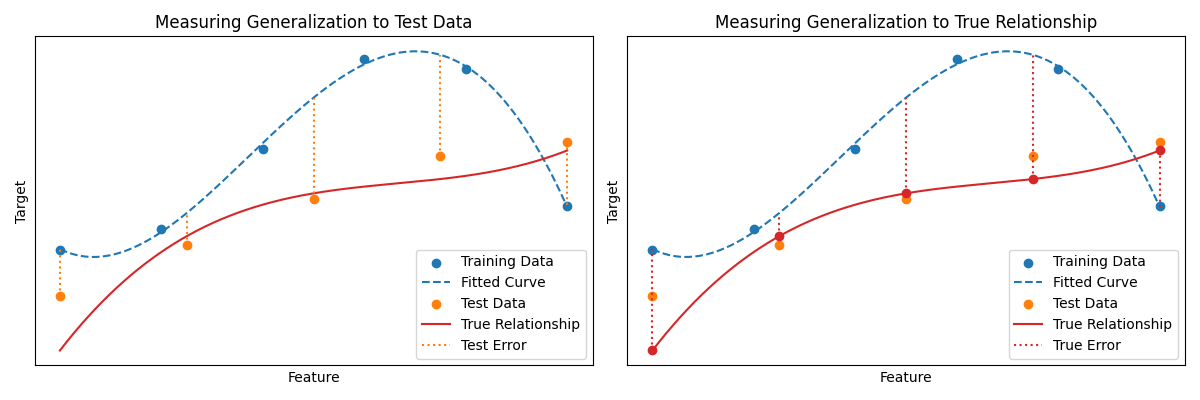
\includegraphics[width=0.8\textwidth]{./project2/figures/datasets.png}
    \caption{Different Levels of Noise}
    \label{fig:datasets}
\end{figure}

Figure~\ref{fig:datasets} shows datasets with different levels of noise in a typical machine learning setting.
The left panel illustrates the common practice of using a test dataset that is separate from the training dataset that is contaminated with noise.
The right panel shows an alternative approach of using \textit{true labels} generated from the true relationship.
In a simulation context, the true relationship, which is the simulation model that generates the data, is visible to the user.
Even if the true relationship is unknown, we can approximate it using a large number of replications and use it as the true labels.
Comparing the errors of a neural network on the true labels can reveal its true generalization capability and robustness.
Chapter~\ref{chap:project2} provides a detailed study of the generalization capability of \gls{lstm} networks in a simulation environment for risk management of \gls{va} contracts.
Viewing the simulation environment as a data-generating process allows us to systematically study and evaluate the performance of neural networks within a controlled setting.
This approach provides insights into their applicability in real-world risk management applications.

In the subsequent chapters, we dive deeper into these topics.
Chapter~\ref{chap:project1} provides a comprehensive analysis of the convergence properties of existing nested simulation procedures and their practical implications.
Chapter~\ref{chap:project2} focuses on the development and evaluation of neural network metamodels, particularly \gls{lstm} networks, for enhancing the efficiency of nested simulations in risk management of \gls{va} contracts.
We also examine the robustness and generalization capabilities of these models in the presence of simulation noise.
Chapter~\ref{chap:project3} explores the use of transfer learning techniques to adapt neural network metamodels to new market conditions and contract specifications.
Our approach enables rapid deployment in changing environments.
Chapter~\ref{chap:conclusion} summarizes the key findings of this thesis and discusses future research directions that involve the robost use of neural networks in quantitative risk management applications.
Chapter~\ref{chap:futureWork} explores future applications of transfer learning and deep reinforcement learning in the dynamic hedging of \gls{va} contracts.
